\chapter{Electronic Identity}

\section{Introduction}
In some instances, several \textbf{relaying parties}(RPs) may decide
to delelegate the authentication process to a separate enetity,
called \textbf{authentication server} (AS) to perform authN on their
behalf, interanction with the authN client by executing an
authentication protocol(there are several of them), and finally
providing to the RP the authN result in the form of a ticket (or
assertion).

\begin{figure}[H]
  \centering
  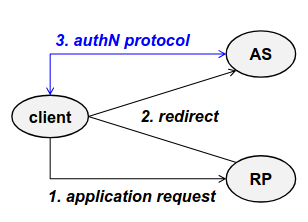
\includegraphics[width=0.5\textwidth]{img/delegated auth.png}
  \caption{Delegated authentication schema}
\end{figure}

At the end of the authN process, the result is trasmitted from the AS
to the RP trough various possible ways, which can vary depending on
various factors:
\begin{itemize}
  \item speed
  \item security and trust
  \item on services, interfaces, network filters
\end{itemize}

\subsection{Possible ticket transmission methods}

% 3 subfigures 
\begin{figure}[H]
  \centering
  \begin{subfigure}{.3\textwidth}
    \centering
    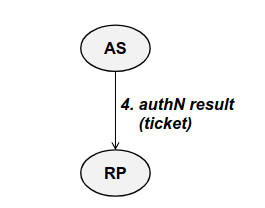
\includegraphics[width=0.9\textwidth]{img/push tickets.png}
    \caption{Push tickets}
  \end{subfigure}
  \begin{subfigure}{.3\textwidth}
    \centering
    \includegraphics[width=0.9\textwidth]{img/inderice push
    tickets.png}
    \caption{Indirect push tickets}
  \end{subfigure}
  \begin{subfigure}{.3\textwidth}
    \centering
    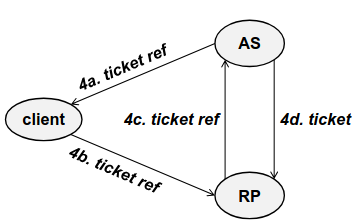
\includegraphics[width=0.9\textwidth]{img/pull ticket.png}
    \caption{Push reference + pull tickets}
  \end{subfigure}
  \caption{Ticket transmission methods}
\end{figure}

\subsection{Problems with tickets}
\begin{itemize}
  \item binding with client
  \item ticket authentication
  \item ticket manipulation (at client)
  \item ticket manipulation (by MITM)
  \item ticket sniffing (in the network / at client) – privacy!
  \item listening service at RP
  \item incoming firewall at RP
  \item ticket replay (by same client): not only when is bound to a
    client, but also if its coming fro mthe same client(identity
    ticket shared among multi user client)
  \item ticket reuse (at different client): is it tied to the client
    or movable to another client?
\end{itemize}

\subsection{Ticket protection}

Ticket protection is essential for securing the transmission of
tickets between the Authentication Server (AS) and the Relying Party
(RP). This protection can be implemented in two primary ways: direct
transmission from AS to RP, and indirect transmission via the client.

\paragraph{Direct Transmission:} 
When tickets are transmitted directly from the AS to the RP, security
can be ensured in one of two ways:
\begin{itemize}
    \item \textbf{Digital Signature and Encryption:} The AS digitally
      signs the ticket and encrypts it specifically for the RP. This
      ensures that only the intended recipient (the RP) can decrypt
      and verify the ticket.
    \item \textbf{Secure Channel:} Alternatively, a secure channel may
      be used, such as TLS, which provides authentication of the AS,
      packet integrity and authentication, packet encryption, and
      protection against replay attacks.
\end{itemize}

\paragraph{Indirect Transmission via Client:}
In cases where tickets are transmitted to the RP through the client,
additional protections are necessary to prevent unauthorized use or
tampering. This approach includes:
\begin{itemize}
    \item \textbf{Digital Signature and Encryption:} The AS digitally
      signs the ticket and encrypts it for the RP, ensuring that it
      can only be decrypted by the RP.
    \item \textbf{Replay Protection:} To prevent replay or reuse of
      tickets, mechanisms such as timestamps can be applied, setting a
      time limit for ticket validity.
    \item \textbf{Binding with Identity and/or Network Address:}
      Tickets can be bound to specific identities or network
      addresses, providing an additional layer of assurance that the
      ticket can only be used by the intended party.
\end{itemize}

These methods collectively contribute to robust ticket protection,
ensuring secure and valid authentication transactions between the AS,
client, and RP.


\subsection{Federated authentication}
Delegate authN are usually inplemanted in a same organization, but it
is possible to federate the authentication among different security
domains, by using a federated authentication system.

This can be done by creating a trust relationship so that a RP
belonging to one domain will accept the authentication performed by
the AS in another domain.

In this case, the authentication server is called \textbf{identity 
provider} (IdP), and the RP is called \textbf{service provider} (SP).
\section{XACML}
XACML (eXtensible Access Control Markup Language) is a language
designed for describing authorization policies and managing access to
protected resources. It defines policies in terms of:

\begin{itemize}
    \item \textbf{Subject:} Entities such as users, computers, or
      services requesting access.
    \item \textbf{Resource:} Items like documents, files, or data that
      are protected and identified through URIs.
\end{itemize}

XACML also includes a language for managing access requests to these
resources. It specifies:

\begin{itemize}
    \item A structured data format to represent access request and
      response messages.
    \item Transmission over a client-server protocol of choice.
\end{itemize}

XACML is an OASIS standard, with its syntax based on XML, making it
widely compatible for authorization tasks in distributed environments.

\subsection{Components policy-based access control}
There are 4 components in a XACML:
\begin{itemize}
  \item  PEP = Policy Enforcement Point: protects a resource and
    allows access only after verification of compatibility with the
    policy
  \item  PDP = Policy Decision Point: receives all the data (policy,
    subject, resource, access type, context) and decides whether to
    permit or deny the access
  \item PIP = Policy Information Point: provides the info related to
    the access requested
  \item PAP = Policy Access Point: provides the policy applicable to
    the requested access
\end{itemize}

\subsection{Policy-base access control architecture}

\begin{figure}[H]
  \centering
  \includegraphics[width=0.5\textwidth]{img/policy access
  control.png}
  \caption{Policy-based access control architecture}
\end{figure}

\subsection{XACML policy format}

\begin{figure}[H]
  \centering
  \includegraphics[width=0.5\textwidth]{img/xacml policy
  format.png}
  \caption{XACML policy format}
\end{figure}


\section{SAML}

SAML (Security Assertion Markup Language) is a data format used for
handling authorization and authentication assertions. It is designed
to:

\begin{itemize}
  \item Represent different types of assertions.
  \item Construct requests for assertions.
  \item Represent responses containing assertions.
\end{itemize}

The core concept in SAML is the \textbf{Assertion}, which serves as
the base object to convey authentication and authorization decisions.
SAML aims to standardize and simplify interactions required to
establish permissions across a multi-domain distributed system.

SAML is an OASIS standard with syntax based on XML. It also provides
online tools to encode and decode various SAML formats and messages. A
helpful tool for this purpose can be found at:
\url{https://www.samltool.com/online_tools.php}

\subsection{SAML 1.\*}

\subsection{SAML 2.0}

\subsection{Use cases}

\subsection{SAML Assertion}

A SAML assertion is a \textbf{declaration of a fact} regarding a
subject, such as the role of a user, made by a specific issuer. There
are three primary types of assertions related to security:

\begin{itemize}
    \item \textbf{Authentication}: confirms the identity of the
      subject.
    \item \textbf{Authorization Decision}: declares whether the
      subject is allowed to access a specific resource.
    \item \textbf{Attributes}: provides additional information about
      the subject, like roles or permissions.
\end{itemize}

SAML assertions are extensible, allowing for the addition of new
assertion types as needed which can be used in a closed domain.
Additionally, assertions can be digitally signed using XML signature
to ensure authenticity and integrity.

\subsubsection{Information Common to All Assertions}

All SAML assertions contain the following common information:

\begin{itemize}
    \item \textbf{Issuer and Issuance Timestamp} – identifies the
      issuer and the exact time the assertion was issued.
    \item \textbf{Assertion ID} – a unique identifier for each
      assertion.
    \item \textbf{Subject} – includes the subject's name and the
      associated security domain.
    \item \textbf{Conditions} – specifies conditions under which the
      assertion is valid:
    \begin{itemize}
        \item SAML clients must reject assertions with conditions they
          do not understand.
        \item An essential condition is the \textit{assertion validity
          period}.
    \end{itemize}
    \item \textbf{Other Useful Information} – may include an
      explanation or proof of the basis on which the assertion was
      constructed.
\end{itemize}

\subsubsection{Authentication Assertion}

An authentication assertion allows an issuer to declare the following
information:

\begin{itemize}
    \item \textbf{Subject (S)} – the subject being authenticated.
    \item \textbf{Mechanism (M)} – the method used for authentication.
    \item \textbf{Time (T)} – the exact time of authentication.
\end{itemize}

\begin{boxH}
  SAML itself does not perform the authentication process (such as
  password requests or challenge-response interactions). Instead, it
  provides a mechanism to link to the results of an authentication
  that has already been completed by an authentication agent.
\end{boxH}


\begin{figure}[H]
  \centering
  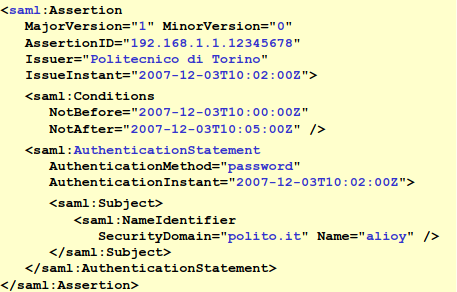
\includegraphics[width=0.6\textwidth]{img/saml auth assertion.png}
  \caption{SAML authentication assertion}
\end{figure}

\subsubsection{Attribute Assertion}

An attribute assertion allows an issuer to declare the following
information:

\begin{itemize}
    \item \textbf{Subject (S)} – the subject associated with specific
      attributes.
    \item \textbf{Attributes (A, B, C, ...)} – a set of attributes
      linked to the subject.
    \item \textbf{Attribute Values} – the current values for each
      attribute, such as "a", "b", "c", etc.
\end{itemize}

\noindent These attributes are typically obtained through an LDAP
query.

\noindent \textbf{Example:} The subject "alioy" within the domain
"polito.it" is associated with the attribute "Department," holding the
value "DAUIN."

\begin{figure}[H]
  \centering
  \includegraphics[width=0.6\textwidth]{img/saml attribute
  assertion.png}
  \caption{SAML attribute assertion}
\end{figure}

\subsubsection{Authorization decision assertion}

\subsection{SAML producer-consumer model}

\begin{figure}[H]
  \centering
  \includegraphics[width=0.6\textwidth]{img/saml produce-consumer
  model.png}
  \caption{SAML producer-consumer model}
\end{figure}



\section{eIDAS}

\section{SPID}

\section{Q\&A}
\subsection*{Question 1}
what role does the Authentication Server (AS) play?
\begin{itemize}
  \incorrect provides authorization decisions for the RP
  \correct performs authentication on behalf of the Relying Party (RP)
  \incorrect verifies the identity of the RP
  \incorrect issues a session timeout for the RP
\end{itemize}

\subsection*{Question 2}
\begin{itemize}
  \incorrect relaying party is A. the entity that directly authenticates the user 
  \incorrect  the server that stores user credentials
  \correct  the entity that trusts another server to handle authentication
  \incorrect  the client application used by the user
\end{itemize}

\subsection*{Question 3}
the Authentication Server (AS) interacts with the client using
specific protocols to perform authentication. What amongst the
following can be used for the authentication process
\begin{itemize}
  \incorrect HTTP 
  \correct OAuth 
  \incorrect FTP
  \incorrect SMTP 
  \correct SAML 
  \incorrect SOAP
\end{itemize}

\subsection*{Question 4}
how does the Authentication Server (AS) typically
communicate the authentication result to the Relying Party (RP)?
\begin{itemize}
  \incorrect  by issuing an authorization code 
  \incorrect  by sending a cookie
  \correct  by providing a ticket or assertion 
  \incorrect  by creating a session ID
\end{itemize}

\subsection*{Question 5}
Which of the following scenarios best represents a delegated authentication setup in a Single Sign-On (SSO) environment
\begin{itemize}
  \incorrect  the user logs in separately to each application with the same credentials
  \correct the user logs in once, and a central AS authenticates them for multiple RPs
  \incorrect each application has its own AS that verifies the user separately
  \incorrect the user must verify their identity with each RP individually
\end{itemize}

\subsection*{Question 6}
Which format is commonly used to provide assertions in delegated authentication systems like SAML?
\begin{itemize}
  \incorrect  JSON Web Tokens (JWT)
  \incorrect  Hypertext Markup Language (HTML) 
  \correct  Extensible Markup Language (XML) 
  \incorrect  Simple Mail Transfer Protocol (SMTP)
\end{itemize}

\subsection*{Question 7}
Which of the following is a key benefit of using delegated authentication for a Relying Party (RP)?
\begin{itemize}
  \incorrect  reduced dependency on external servers 
  \correct  enhanced data privacy for user credentials 
  \incorrect  increased complexity in user management 
  \incorrect  independent authentication for each RP
\end{itemize}

\subsection*{Question 8}
what does a SAML assertion represent?
\begin{itemize}
  \correct  declaration of a fact about a subject, like user information
  \incorrect  a statement about of how often a user logs in
  \incorrect  a protocol for secure email communication
  \incorrect  a form of encryption used for securing passwords
  \incorrect  a method of encoding data in XML format
  \correct  declaration made by an issuer about a different subject
\end{itemize}

\subsection*{Question 9}
Which of the following is not a standard type of SAML assertion?
\begin{itemize}
  \incorrect  authentication assertion
  \correct  Service type assertion
  \incorrect  authorization decision assertion 
  \correct  public key certificate assertion 
  \incorrect  attribute assertion
  \correct  token assertion
\end{itemize}

\subsection*{Question 10}
When an Identity Provider (IdP) issues a SAML assertion, who is
typically the recipient that relies on this assertion?
\begin{itemize}
  \incorrect user's web browser
  \correct Relying Party (RP)
  \correct Service Provider (SP)
  \incorrect DNS server
  \incorrect certificate authority 
  \incorrect password manager
\end{itemize}

\subsection*{Question 11}
Why does SAML use XML as the standard format for its assertions?
\begin{itemize}
  \correct  XML provides a flexible, readable format for exchanging
  information across systems
  \incorrect  XML is universally adored by data specialists 
  \incorrect  XML is the default because JSON was too complicated
  \correct  XML allows for custom-defined tags, which means SAML can
  extend its structure to include additional fields or attributes as
  needed without breaking compatibility with existing systems
  \incorrect  XML prevents other formats from being easily implemented 
  \incorrect  XML encodes information only in binary for extra security
  \correct  XML allows SAML to be platform-independent and easily
  parsed by different systems 
\end{itemize}

\subsection*{Question 12}
In policy-based access control (PBAC), what is the primary function of
the Policy Enforcement Point (PEP)?
\begin{itemize}
  \correct enforces access to a resource based on the policy decision 
  \incorrect collects user attributes for policy decision-making
  \incorrect decides whether a policy is applicable to a specific
  access request
  \incorrect acts as a backup in case the Policy Decision Point (PDP)
  fails
  \incorrect protects resources by ensuring they're only accessed when
  policies align with user attributes
\end{itemize}

\subsection*{Question 13}
Which of the following best describes the role of the Policy Decision
Point (PDP) in PBAC?
\begin{itemize}
  \incorrect enforces access controls based on predefined policies
  \incorrect collects and provides the necessary policies for the reguested access
  \correct evaluates all information (policy, subject, resource, and access type) to determine if access should be granted
  \incorrect monitors user behavior and access patterns for anomaly detection
  \incorrect checks user permissions, but only on days when its not overloaded
  \incorrect none of the above
\end{itemize}

\subsection*{Question 14}
What is the primary purpose of a SAML binding?
\begin{itemize}
  \correct to specify the underlying protocol used to transport SAML
  reguests and responses
  \incorrect to define how SAML assertions are signed for security purposes
  \incorrect to describe the format of SAML messages exchanged between
  systems
  \incorrect to establish a fallback protocol for non-compliant systems
  \incorrect to ensure SAML messages are transported using the fastest
  possible route
\end{itemize}

\subsection*{Question 15}
Which of the following is not a valid SAML binding?
\begin{itemize}
  \incorrect  SAML SOAP binding
  \incorrect Reverse SOAP (PAOS) binding
  \incorrect  HTTP POST binding
  \correct FTP-over-SAML binding
  \incorrect  HTTP redirect binding
  \correct  SAML-over-TLS binding
\end{itemize}

\subsection*{Question 16}
In the SAML SOAP binding, what role does SOAP play?
\begin{itemize}
  \incorrect  It formats the SAML reguest/response messages in XML for
  transmission
  \incorrect  It determines the security of the SAML assertion being
  transported
  \correct  It wraps SAML messages inside a SOAP envelope over HTTP
  \incorrect  It acts as an intermediary to deliver SAML assertions
  across different servers
  \incorrect  It ensures messages are "clean and shiny" before they'Tre
  sent
\end{itemize}
